\documentclass[margin=.4in]{paper}

\usepackage{graphicx}

\title{Social Engineering \& Fraud Detection}

\graphicspath{{graphics/}}

\begin{document}
	\maketitle
	
	\section{Introduction}
	
	The paper mainly focuses on how to deliver a detection for Fraud detection. The approach taken is by analyzing content of the messages and detecting inappropriate statements in the attacker commands.
	
	Likely the paper have taken the approach the message by dividing all statements that could be suspicious to be either two things for first part (A):
	
	\begin{enumerate}
		\item[A. ] \begin{itemize}
			\item \textbf{Ask} a private request that results in the disclosure of sensitive information; An technique based on paper for detecting improper queries uses research in question answering systems to establish the privacy of the attacker's replies to questions.
			\item \textbf{Issue} a command to do an unlawful activity; the strategy is to evaluate instructions by combining the primary verb and the object(s) of that verb in the phrase to summarize their meaning.
		\end{itemize}
	
		\item[B. ] The data set are collected from real social engineering attacks the also required for effectiveness of paper approach.
	\end{enumerate}

	The main steps are configured as follows:
	
	\begin{figure}[htbp]
		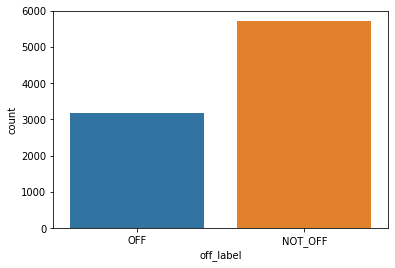
\includegraphics[width=\columnwidth, height=.1\textheight]{01.png}
		\caption{Illustration of the approach}
	\end{figure}


	\clearpage
	
	\section{Sentence Processing}
	The message is processed by dividing words into sentences and parse each single sentence to find an informative pattern which is helpful for analysis. The operation is made by using an online punctuation tool to make sure each is well understood by the model.
	
	\section{\textsc{Sentence Type Identifications}}
	
	Questions and commands are the types of sentences that declared we are focusing on because they might issue a private manner for the victim in which the attacker wants to reveal info about. 
	
	And there are four types of commands that are we concerned about:
	
	\begin{itemize}
		\item \textbf{Direct imperatives} - They are made using imperative type of sentence which starts with a verb like ``Open the door" or ``Come in".
		\item \textbf{Polite prefixes} - It is at first looks like to be imperative but in the heart it is rude. (e. g.) ``Please go home"
		\item \textbf{Suggestion} - Rather than telling a person what to do, you may tell them what to do.
		If the order is to have the victim undertake an activity, it may be stated as a suggestion that the victim should follow, such as ``You could open the door".
		\item \textbf{Expression of desire} - Another method to soften a demand is to precede it with a wish expression like ``I want you to come in".
	\end{itemize}
	
	\section{\textsc{Form Identification}}
	Without overtly asking a question, an attacker may ask the victim to answer a question by just stating the data that is sought. As many circumstances, the information sought is delivered in an itemized list that the victim interprets as a series of implicit inquiries depending on the situation.
	And It is divided into two forms ``What is your \texttt{<item>}? " where item is the form item and ``\texttt{<item>}:"
	
	\clearpage
	
	\section{\textsc{Question Analysis}}
	The existing \uppercase{\textbf{paralex}} question answering system which we modified is fully described in previous work and is outlined in paper.
	
	It is briefly identified in figure~\ref{fig:question_analysis}.
	
	\begin{figure}[htbp]
		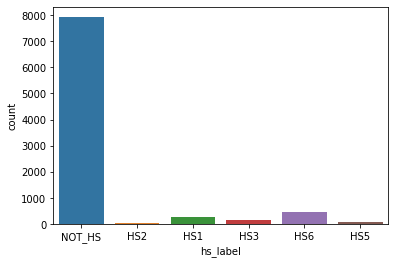
\includegraphics[width=\textwidth, height=.4\columnwidth]{02.png}
		\caption{Searching for a term in database}
		\label{fig:question_analysis}
	\end{figure}

\end{document}